\documentclass{standalone}
\usepackage{tikz}
\usetikzlibrary{patterns, positioning}
\usepackage[sfdefault]{ClearSans} %% option 'sfdefault' activates Clear Sans as the default text font
\usepackage[T1]{fontenc}

\begin{document}
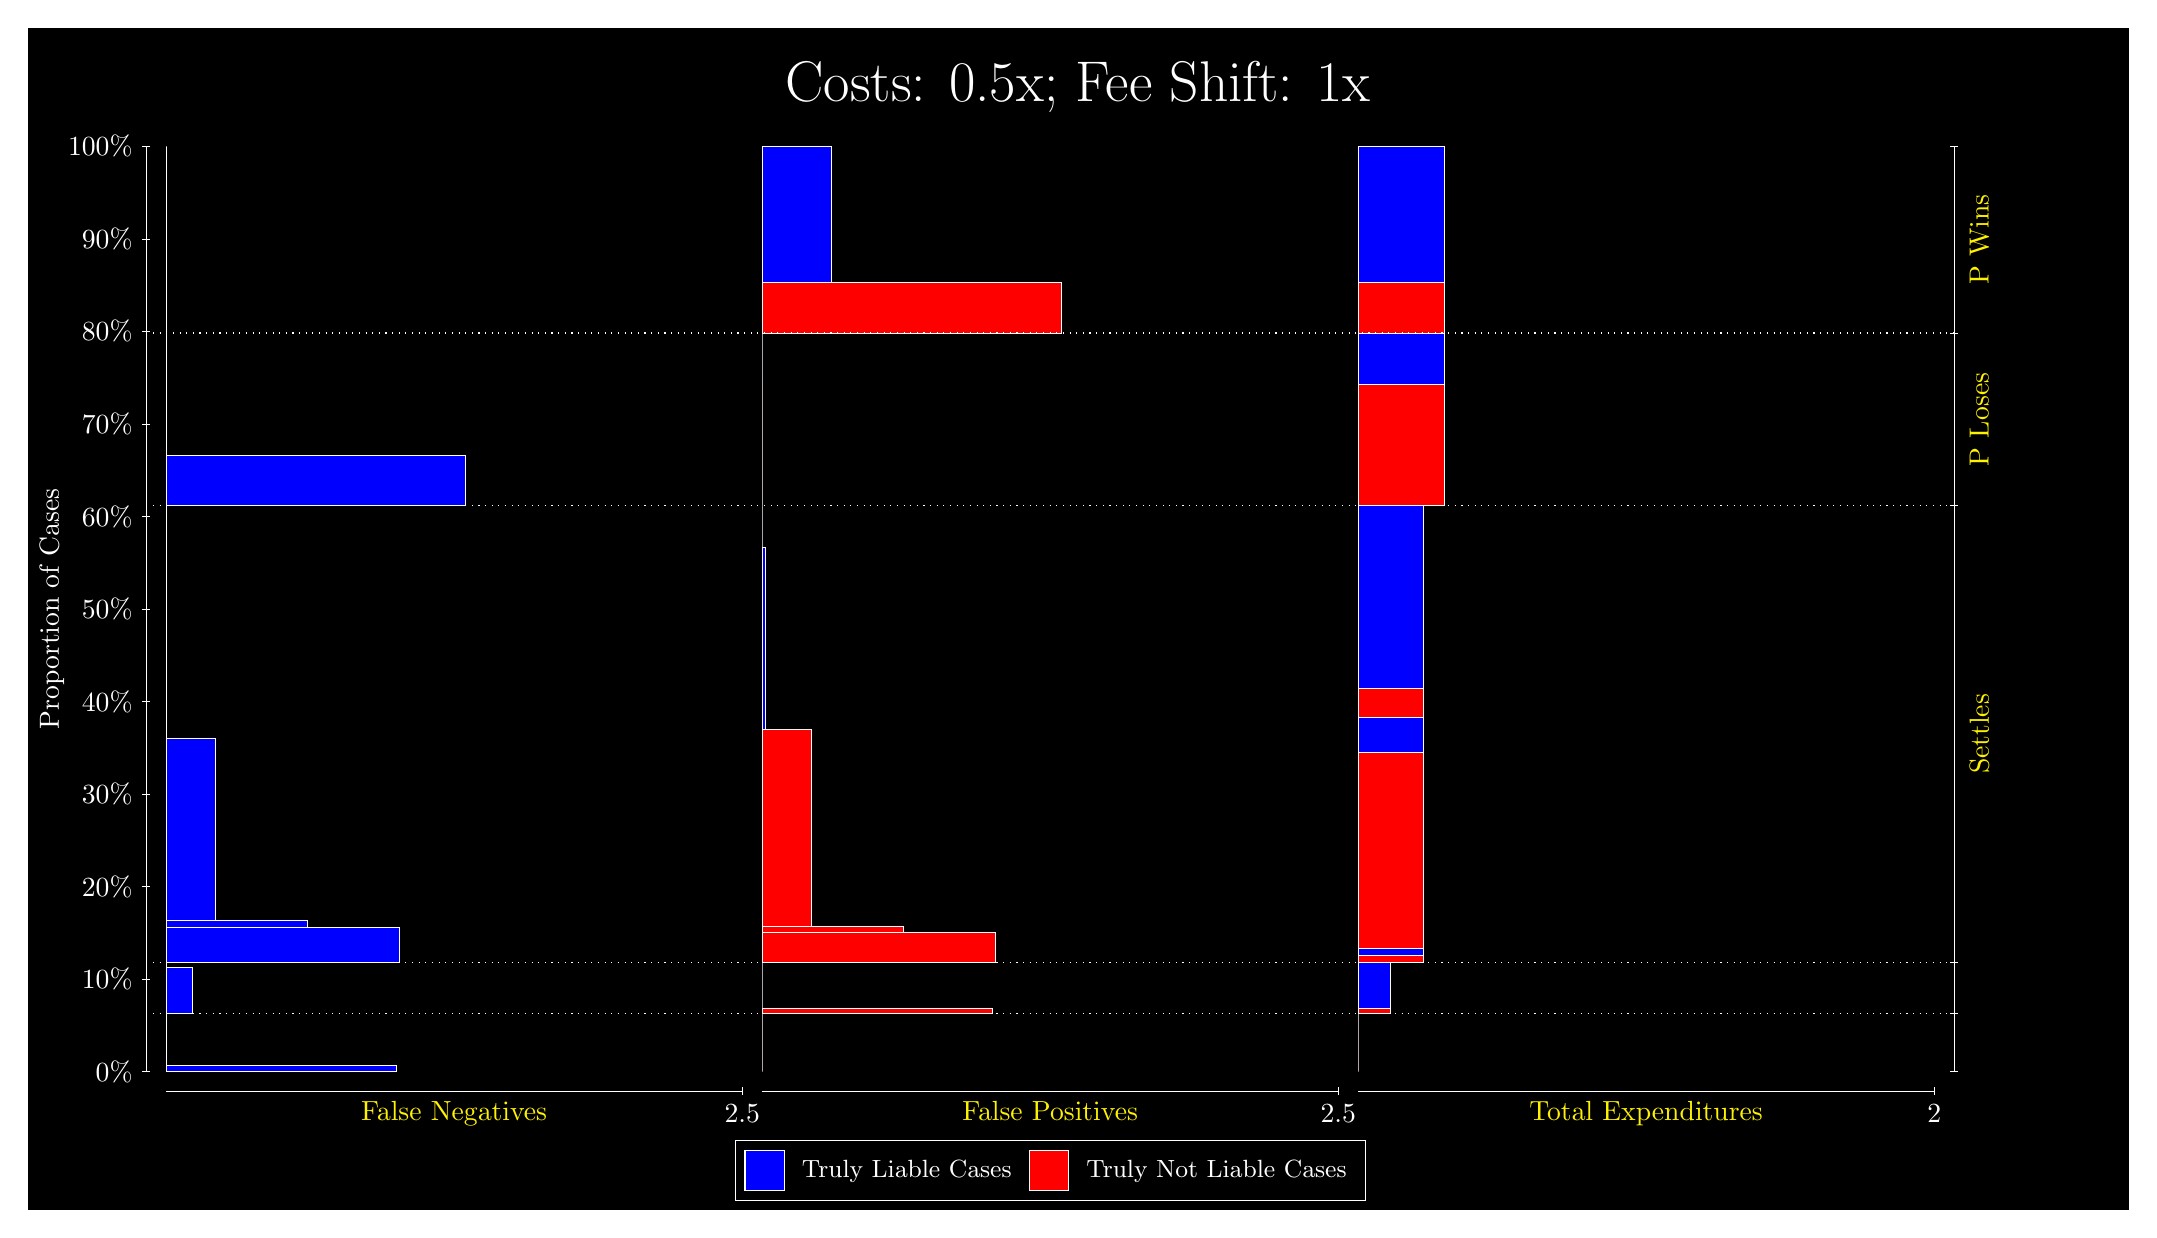
\begin{tikzpicture}
\draw[fill=black] (0,0) rectangle (26.667,15);
\draw[text=white] (0,13.5) rectangle (26.667,15) node[midway] {\huge Costs: 0.5x; Fee Shift: 1x};
\draw[white, very thin] (1.5,1.75) -- (1.5,13.5);
\node[rotate=90, text=white, anchor=center] at (0.3, 7.625) {Proportion of Cases};
\draw[white, very thin] (1.45,1.75) -- (1.55,1.75);
\node[text=white, anchor=east] at (1.45, 1.75) {0\%};
\draw[white, very thin] (1.45,2.925) -- (1.55,2.925);
\node[text=white, anchor=east] at (1.45, 2.925) {10\%};
\draw[white, very thin] (1.45,4.1) -- (1.55,4.1);
\node[text=white, anchor=east] at (1.45, 4.1) {20\%};
\draw[white, very thin] (1.45,5.275) -- (1.55,5.275);
\node[text=white, anchor=east] at (1.45, 5.275) {30\%};
\draw[white, very thin] (1.45,6.45) -- (1.55,6.45);
\node[text=white, anchor=east] at (1.45, 6.45) {40\%};
\draw[white, very thin] (1.45,7.625) -- (1.55,7.625);
\node[text=white, anchor=east] at (1.45, 7.625) {50\%};
\draw[white, very thin] (1.45,8.8) -- (1.55,8.8);
\node[text=white, anchor=east] at (1.45, 8.8) {60\%};
\draw[white, very thin] (1.45,9.975) -- (1.55,9.975);
\node[text=white, anchor=east] at (1.45, 9.975) {70\%};
\draw[white, very thin] (1.45,11.15) -- (1.55,11.15);
\node[text=white, anchor=east] at (1.45, 11.15) {80\%};
\draw[white, very thin] (1.45,12.325) -- (1.55,12.325);
\node[text=white, anchor=east] at (1.45, 12.325) {90\%};
\draw[white, very thin] (1.45,13.5) -- (1.55,13.5);
\node[text=white, anchor=east] at (1.45, 13.5) {100\%};

\draw[white, very thin] (24.457,1.75) -- (24.457,13.5);
\draw[white, very thin] (24.407,1.75) -- (24.507,1.75);
\node[anchor=west] at (24.407, 1.75) {};
\draw[white, very thin] (24.407,2.4848) -- (24.507,2.4848);
\node[anchor=west] at (24.407, 2.4848) {};
\draw[white, very thin] (24.407,3.1397) -- (24.507,3.1397);
\node[anchor=west] at (24.407, 3.1397) {};
\draw[white, very thin] (24.407,8.9363) -- (24.507,8.9363);
\node[anchor=west] at (24.407, 8.9363) {};
\draw[white, very thin] (24.407,11.129) -- (24.507,11.129);
\node[anchor=west] at (24.407, 11.129) {};
\draw[white, very thin] (24.407,13.5) -- (24.507,13.5);
\node[anchor=west] at (24.407, 13.5) {};

\draw[white, very thin, fill=blue] (1.75,1.75) rectangle (4.6775,1.8273);
\draw[white, very thin, fill=red] (1.75,1.8273) rectangle (1.75,2.4848);
\draw[white, very thin, fill=blue] (1.75,2.4848) rectangle (2.0793,3.0715);
\draw[white, very thin, fill=red] (1.75,3.0715) rectangle (1.75,3.1397);
\draw[white, very thin, fill=blue] (1.75,3.1397) rectangle (4.7141,3.5781);
\draw[white, very thin, fill=blue] (1.75,3.5781) rectangle (3.5431,3.6652);
\draw[white, very thin, fill=blue] (1.75,3.6652) rectangle (2.3721,5.9801);
\draw[white, very thin, fill=red] (1.75,5.9801) rectangle (1.75,8.9363);
\draw[white, very thin, fill=blue] (1.75,8.9363) rectangle (5.5558,9.5818);
\draw[white, very thin, fill=red] (1.75,9.5818) rectangle (1.75,11.129);
\draw[white, very thin, fill=red] (1.75,11.129) rectangle (1.75,11.775);
\draw[white, very thin, fill=blue] (1.75,11.775) rectangle (1.75,13.5);
\draw[white, very thin, fill=red] (9.3189,1.75) rectangle (9.3189,2.4075);
\draw[white, very thin, fill=blue] (9.3189,2.4075) rectangle (9.3189,2.4848);
\draw[white, very thin, fill=red] (9.3189,2.4848) rectangle (12.246,2.5531);
\draw[white, very thin, fill=blue] (9.3189,2.5531) rectangle (9.3189,3.1397);
\draw[white, very thin, fill=red] (9.3189,3.1397) rectangle (12.283,3.5165);
\draw[white, very thin, fill=red] (9.3189,3.5165) rectangle (11.112,3.6);
\draw[white, very thin, fill=red] (9.3189,3.6) rectangle (9.941,6.0959);
\draw[white, very thin, fill=blue] (9.3189,6.0959) rectangle (9.3555,8.4108);
\draw[white, very thin, fill=blue] (9.3189,8.4108) rectangle (9.3189,8.9363);
\draw[white, very thin, fill=red] (9.3189,8.9363) rectangle (9.3189,10.483);
\draw[white, very thin, fill=blue] (9.3189,10.483) rectangle (9.3189,11.129);
\draw[white, very thin, fill=red] (9.3189,11.129) rectangle (13.125,11.775);
\draw[white, very thin, fill=blue] (9.3189,11.775) rectangle (10.197,13.5);
\draw[white, very thin, fill=red] (16.888,1.75) rectangle (16.888,2.4075);
\draw[white, very thin, fill=blue] (16.888,2.4075) rectangle (16.888,2.4848);
\draw[white, very thin, fill=red] (16.888,2.4848) rectangle (17.299,2.5531);
\draw[white, very thin, fill=blue] (16.888,2.5531) rectangle (17.299,3.1397);
\draw[white, very thin, fill=red] (16.888,3.1397) rectangle (17.711,3.2233);
\draw[white, very thin, fill=blue] (16.888,3.2233) rectangle (17.711,3.3103);
\draw[white, very thin, fill=red] (16.888,3.3103) rectangle (17.711,5.8062);
\draw[white, very thin, fill=blue] (16.888,5.8062) rectangle (17.711,6.2446);
\draw[white, very thin, fill=red] (16.888,6.2446) rectangle (17.711,6.6213);
\draw[white, very thin, fill=blue] (16.888,6.6213) rectangle (17.711,8.9363);
\draw[white, very thin, fill=red] (16.888,8.9363) rectangle (17.986,10.483);
\draw[white, very thin, fill=blue] (16.888,10.483) rectangle (17.986,11.129);
\draw[white, very thin, fill=red] (16.888,11.129) rectangle (17.986,11.775);
\draw[white, very thin, fill=blue] (16.888,11.775) rectangle (17.986,13.5);
\draw[white, dotted] (1.5,2.4848) -- (24.457,2.4848);
\draw[white, dotted] (1.5,3.1397) -- (24.457,3.1397);
\draw[white, dotted] (1.5,8.9363) -- (24.457,8.9363);
\draw[white, dotted] (1.5,11.129) -- (24.457,11.129);
\draw[white, very thin] (1.75,1.5) -- (9.0689,1.5);
\node[text=yellow, anchor=north] at (5.4094, 1.5) {False Negatives};
\draw[white, very thin] (9.0689,1.45) -- (9.0689,1.55);
\node[text=white, anchor=north] at (9.0689, 1.45) {2.5};

\draw[white, very thin] (9.3189,1.5) -- (16.638,1.5);
\node[text=yellow, anchor=north] at (12.978, 1.5) {False Positives};
\draw[white, very thin] (16.638,1.45) -- (16.638,1.55);
\node[text=white, anchor=north] at (16.638, 1.45) {2.5};

\draw[white, very thin] (16.888,1.5) -- (24.207,1.5);
\node[text=yellow, anchor=north] at (20.547, 1.5) {Total Expenditures};
\draw[white, very thin] (24.207,1.45) -- (24.207,1.55);
\node[text=white, anchor=north] at (24.207, 1.45) {2};



\node[text=yellow, centered, rotate=90] at (24.777, 6.038) {Settles};
\node[text=yellow, centered, rotate=90] at (24.777, 10.032) {P Loses};
\node[text=yellow, centered, rotate=90] at (24.777, 12.314) {P Wins};

\draw (12.978300999999998,1.5) node[draw=none] (baseCoordinate) {};
\begin{scope}[align=center]
        \matrix[scale=0.5, draw=white, below=0.5cm of baseCoordinate, nodes={draw}, column sep=0.1cm]{
            \node[rectangle, draw, minimum width=0.5cm, minimum height=0.5cm, fill=blue] {}; &
            \node[draw=none, font=\small, text=white] (B) {Truly Liable Cases}; &
            \node[rectangle, draw, minimum width=0.5cm, minimum height=0.5cm, fill=red] {}; &
            \node[draw=none, font=\small, text=white] (B) {Truly Not Liable Cases}; \\
            };
\end{scope}

\end{tikzpicture}
\end{document}